% Reporte ejecutivo de la entrega final (entrega 2).
%
% Es incremental: el enunciado pide incluir los resultados de la primera entrega
% (secciones 1 a 7) ajustados según las recomendaciones recibidas. Esas secciones
% parten del texto de entrega-1/reporte/reporte.tex; al comienzo de cada una, un
% comentario resume lo que dijo la rúbrica de los docentes (el detalle está en
% entrega-1/retroalimentacion.md). Las secciones 8 a 13 son nuevas.
%
% Formato que exige el enunciado: PDF, una columna, Arial 12, máximo 12 páginas,
% enfoque netamente ejecutivo y con enlaces a los recursos del repositorio donde
% está el detalle. El enunciado recomienda no gastar páginas en portada ni tabla de
% contenidos; la portada se puede quitar con \portadafalse.
%
% Se compila con LuaLaTeX (hace falta para usar Arial), desde esta carpeta:
%
%     latexmk reporte.tex
%
\documentclass[12pt,letterpaper]{article}

\newcommand{\titulo}{Transición predial 2027: un producto de datos para fijar tarifas después de la actualización catastral}
\newcommand{\titulocorto}{Transición predial 2027} % va en la franja de cada página
\newcommand{\subtitulo}{Escenarios de tarifas y límites del impuesto predial 2027 para un municipio colombiano, con Multiaservi Consultores}
\newcommand{\entrega}{Entrega final}
\newcommand{\fecha}{Bogotá, noviembre de 2026}
\newcommand{\maxpaginas}{12}
\newcommand{\urlrepositorio}{https://github.com/Danielfts/proyecto-MINE-ciencia-de-datos}
% Pendiente: el enlace del video de la entrega final en YouTube
\newcommand{\urlvideo}{https://www.youtube.com/}
% Archivo de predios en el almacenamiento de la Universidad (acceso restringido)
\newcommand{\urldatos}{https://uniandes-my.sharepoint.com/:u:/r/personal/d_trivino_uniandes_edu_co/Documents/CollegeSemesters/2026_2/Ciencia\%20de\%20Datos/datasets/predios.parquet?d=w86352a73a04e416d8149f8782df4e840\&csf=1\&web=1\&e=jxKQvW}

% Colores, tipografía, encabezado, portada y enlaces: identidad/estilo-reporte.tex.
% Integrantes de la entrega final, en el orden del README
\newcommand{\integrantesportada}{Daniel Felipe Triviño Santana\\ Nicolas Bedoya Figueroa\\
  Joubert Daniel Álvarez\\ Gabriel Bejarano}
\newcommand{\integrantescompacto}{Daniel Felipe Triviño Santana, Nicolas Bedoya Figueroa,\\
  Joubert Daniel Álvarez, Gabriel Bejarano}

% Estilo de los reportes del proyecto, con la identidad visual de la Universidad
% de los Andes: amarillo, negro y blanco, y tipografía sin serifas (ver README.md
% de esta carpeta). Lo comparten los reportes de las dos entregas.
%
% El reporte define antes: \titulo, \titulocorto, \subtitulo, \entrega, \fecha,
% \urlrepositorio, \urlvideo y \maxpaginas, y pone % Estilo de los reportes del proyecto, con la identidad visual de la Universidad
% de los Andes: amarillo, negro y blanco, y tipografía sin serifas (ver README.md
% de esta carpeta). Lo comparten los reportes de las dos entregas.
%
% El reporte define antes: \titulo, \titulocorto, \subtitulo, \entrega, \fecha,
% \urlrepositorio, \urlvideo y \maxpaginas, y pone % Estilo de los reportes del proyecto, con la identidad visual de la Universidad
% de los Andes: amarillo, negro y blanco, y tipografía sin serifas (ver README.md
% de esta carpeta). Lo comparten los reportes de las dos entregas.
%
% El reporte define antes: \titulo, \titulocorto, \subtitulo, \entrega, \fecha,
% \urlrepositorio, \urlvideo y \maxpaginas, y pone \input{../../identidad/estilo-reporte}.
% Puede definir también los integrantes: \integrantesportada (un nombre por línea, para
% la portada) e \integrantescompacto (para el título compacto). Si no, salen los tres
% de la primera entrega.
% Se compila con LuaLaTeX.

\providecommand{\integrantesportada}{Daniel Felipe Triviño Santana\\ Nicolas Bedoya Figueroa\\
  Joubert Daniel Álvarez}
\providecommand{\integrantescompacto}{Daniel Felipe Triviño Santana, Nicolas Bedoya Figueroa,\\
  Joubert Daniel Álvarez}

\usepackage[spanish,es-tabla,es-nodecimaldot]{babel}
\usepackage{fontspec}
\usepackage[letterpaper,left=2.5cm,right=2.5cm,top=2.6cm,bottom=2.4cm,
  headheight=15pt,headsep=0.8cm,footskip=1.0cm]{geometry}
\usepackage{graphicx}
\usepackage{booktabs}
\usepackage{enumitem}
\usepackage{titlesec}
\usepackage{csquotes}
\usepackage{xcolor}
\usepackage{luacolor}
\usepackage{lua-ul}
\usepackage{tikz}
\usepackage{fancyhdr}
\usepackage{lastpage}
\usepackage[font=small,labelfont=bf,labelsep=period]{caption}
\usepackage[backend=biber,style=numeric,sorting=none]{biblatex}
\usepackage[hidelinks]{hyperref}

\newcommand{\dirIdentidad}{../../identidad}

% --- Colores -----------------------------------------------------------------
% Los oficiales del logosímbolo: negro y amarillo (C0 M0 Y100 K0). El amarillo se
% define en CMYK para que sea exactamente el del logo.
\definecolor{amarillo}{cmyk}{0,0,1,0}
\colorlet{negro}{black}
\definecolor{gris}{gray}{0.40}
\definecolor{grisclaro}{gray}{0.94}

% --- Tipografía --------------------------------------------------------------
% Arial 12 (lo exige el enunciado; el manual recomienda fuentes sin serifas). Si
% Arial no está instalada se usa una fuente con las mismas medidas, para que el
% número de páginas no cambie, pero el PDF que se entrega debe salir con Arial.
\IfFontExistsTF{Arial}{\setmainfont{Arial}}{%
  \IfFontExistsTF{Liberation Sans}{\setmainfont{Liberation Sans}}{\setmainfont{TeX Gyre Heros}}%
  \AtEndDocument{\PackageWarningNoLine{reporte}{Arial no esta instalada: este PDF usa una
    fuente sustituta. Compile la version que se entrega en un equipo con Arial}}}
\renewcommand{\familydefault}{\rmdefault}

% --- Títulos, listas y párrafos: compactos, el espacio es para el contenido -----
\titleformat{\section}{\large\bfseries}
  {\colorbox{amarillo}{\makebox[1.3em]{\strut\thesection}}}{0.6em}{}
\titleformat{\subsection}{\normalsize\bfseries}{\thesubsection}{0.5em}{}
\titlespacing*{\section}{0pt}{1.4ex plus 0.4ex}{0.7ex}
\titlespacing*{\subsection}{0pt}{1ex plus 0.3ex}{0.4ex}
\setlist{nosep,leftmargin=*}
\setlist[itemize,1]{label=\textcolor{amarillo}{\rule[0.15ex]{0.9ex}{0.9ex}}}
\setlength{\parskip}{0.5ex}
\setlength{\parindent}{0pt}

% --- Enlaces: texto negro con subrayado amarillo ---------------------------------
\newcommand{\enlace}[2]{\href{#1}{\underLine[color=amarillo,top=-0.22ex,bottom=-0.42ex]{#2}}}
% Enlace a un archivo o carpeta del repositorio: \repo{ruta/al/archivo}{texto}.
\newcommand{\repo}[2]{\enlace{\urlrepositorio/blob/main/#1}{#2}}

% --- Recuadro para el resultado o la cifra que no se puede pasar por alto --------
% Fondo gris con una barra amarilla a la izquierda. No se parte entre páginas.
\newsavebox{\cajadestacado}
\newenvironment{destacado}{%
  \par\addvspace{1.2ex}\noindent\setlength{\fboxsep}{6pt}%
  \begin{lrbox}{\cajadestacado}%
  \begin{minipage}{\dimexpr\linewidth-3pt-2\fboxsep\relax}\setlength{\parskip}{0.5ex}}
  {\end{minipage}\end{lrbox}%
  \textcolor{amarillo}{\vrule width 3pt}\colorbox{grisclaro}{\usebox{\cajadestacado}}%
  \par\addvspace{1.2ex}}

% --- Encabezado y pie de página --------------------------------------------------
% Franja amarilla de borde a borde, con una línea negra debajo.
\newcommand{\franja}{%
  \begin{tikzpicture}[remember picture,overlay]
    \fill[amarillo] (current page.north west) rectangle
      ([yshift=-1.15cm]current page.north east);
    \fill[negro] ([yshift=-1.15cm]current page.north west) rectangle
      ([yshift=-1.21cm]current page.north east);
    \node[anchor=west,font=\small\bfseries,text=negro]
      at ([xshift=2.5cm,yshift=-0.6cm]current page.north west) {\titulocorto};
    \node[anchor=east,font=\small,text=negro]
      at ([xshift=-2.5cm,yshift=-0.6cm]current page.north east) {\entrega};
  \end{tikzpicture}}
\pagestyle{fancy}
\fancyhf{}
\fancyhead[L]{\franja}
\fancyfoot[L]{\footnotesize\color{gris}MINE-4101 Ciencia de Datos Aplicada · Universidad de los Andes}
\fancyfoot[R]{\footnotesize\color{gris}\thepage\ de \pageref*{LastPage}}
\renewcommand{\headrulewidth}{0pt}
\renewcommand{\footrulewidth}{0.4pt}

% --- Portada ----------------------------------------------------------------------
% El logo a color va sobre blanco, sin modificar y acompañado del texto legal, como
% pide el manual de identidad.
\newcommand{\legaluniandes}{Universidad de los Andes | Vigilada Mineducación.
  Reconocimiento como Universidad: Decreto 1297 del 30 de mayo de 1964.
  Reconocimiento personería jurídica: Resolución 28 del 23 de febrero de 1949 Minjusticia.}

\newcommand{\portada}{%
  \begin{titlepage}
  \begin{tikzpicture}[remember picture,overlay]
    \node[anchor=north west,inner sep=0pt]
      at ([xshift=2.5cm,yshift=-2.2cm]current page.north west)
      {\includegraphics[height=1.9cm]{\dirIdentidad/logo-uniandes.pdf}};
    % bloque amarillo de borde a borde, con el título
    \fill[amarillo] ([yshift=-7.6cm]current page.north west) rectangle
      ([yshift=-16.0cm]current page.north east);
    \node[anchor=north west,inner sep=0pt,text width=16.5cm,align=left]
      at ([xshift=2.5cm,yshift=-8.7cm]current page.north west) {%
        \hyphenpenalty=10000\exhyphenpenalty=10000
        {\small\bfseries\addfontfeature{LetterSpace=12}\MakeUppercase{Proyecto final · \entrega}}\\[0.9cm]
        {\fontsize{30}{35}\selectfont\bfseries\titulo\par}\vspace{0.6cm}
        {\Large\subtitulo\par}};
    % franja negra con el curso
    \fill[negro] ([yshift=-16.0cm]current page.north west) rectangle
      ([yshift=-17.3cm]current page.north east);
    \node[anchor=west,text=white,font=\normalsize\bfseries]
      at ([xshift=2.5cm,yshift=-16.65cm]current page.north west)
      {MINE-4101 Ciencia de Datos Aplicada};
    \node[anchor=east,text=white,font=\normalsize]
      at ([xshift=-2.5cm,yshift=-16.65cm]current page.north east) {Semestre 2026-20};
    % integrantes y profesores
    \node[anchor=north west,inner sep=0pt,text width=8.5cm,align=left]
      at ([xshift=2.5cm,yshift=-18.6cm]current page.north west) {%
        {\small\bfseries\addfontfeature{LetterSpace=12}INTEGRANTES}\\[0.25cm]
        \integrantesportada};
    \node[anchor=north west,inner sep=0pt,text width=7cm,align=left]
      at ([xshift=12cm,yshift=-18.6cm]current page.north west) {%
        {\small\bfseries\addfontfeature{LetterSpace=12}PROFESORES}\\[0.25cm]
        Fabian Camilo Peña\\ Juan Pablo Reyes\\[0.5cm]
        \enlace{\urlrepositorio}{Repositorio} · \enlace{\urlvideo}{Video}\\[0.15cm]
        \fecha};
    % texto legal que acompaña al logo
    \draw[negro,line width=0.4pt] ([xshift=2.5cm,yshift=2.5cm]current page.south west)
      -- ([xshift=-2.5cm,yshift=2.5cm]current page.south east);
    \node[anchor=north west,inner sep=0pt,text width=16.5cm,align=left,
      font=\scriptsize,text=gris]
      at ([xshift=2.5cm,yshift=2.3cm]current page.south west) {\legaluniandes};
  \end{tikzpicture}
  \end{titlepage}
  \setcounter{page}{2}}

% Título compacto, para cuando no hay portada.
\newcommand{\titulocompacto}{%
  \begin{center}
    {\Large\bfseries\titulo\par}\vspace{0.5ex}
    \entrega\ · MINE-4101 Ciencia de Datos Aplicada · 2026-20\\[0.5ex]
    \integrantescompacto\\[0.5ex]
    \enlace{\urlrepositorio}{Repositorio} · \enlace{\urlvideo}{Video de sustentación}
  \end{center}}

% \encabezado pone la portada o, con \portadafalse, el título compacto.
\newif\ifportada
\portadatrue
\newcommand{\encabezado}{\ifportada\portada\else\titulocompacto\fi}

% --- Aviso si el reporte se pasa del máximo de páginas ---------------------------
\AtEndDocument{\ifnum\value{page}>\maxpaginas\relax
  \PackageWarningNoLine{reporte}{El reporte tiene \thepage\space paginas y el maximo
    es \maxpaginas}\fi}
.
% Puede definir también los integrantes: \integrantesportada (un nombre por línea, para
% la portada) e \integrantescompacto (para el título compacto). Si no, salen los tres
% de la primera entrega.
% Se compila con LuaLaTeX.

\providecommand{\integrantesportada}{Daniel Felipe Triviño Santana\\ Nicolas Bedoya Figueroa\\
  Joubert Daniel Álvarez}
\providecommand{\integrantescompacto}{Daniel Felipe Triviño Santana, Nicolas Bedoya Figueroa,\\
  Joubert Daniel Álvarez}

\usepackage[spanish,es-tabla,es-nodecimaldot]{babel}
\usepackage{fontspec}
\usepackage[letterpaper,left=2.5cm,right=2.5cm,top=2.6cm,bottom=2.4cm,
  headheight=15pt,headsep=0.8cm,footskip=1.0cm]{geometry}
\usepackage{graphicx}
\usepackage{booktabs}
\usepackage{enumitem}
\usepackage{titlesec}
\usepackage{csquotes}
\usepackage{xcolor}
\usepackage{luacolor}
\usepackage{lua-ul}
\usepackage{tikz}
\usepackage{fancyhdr}
\usepackage{lastpage}
\usepackage[font=small,labelfont=bf,labelsep=period]{caption}
\usepackage[backend=biber,style=numeric,sorting=none]{biblatex}
\usepackage[hidelinks]{hyperref}

\newcommand{\dirIdentidad}{../../identidad}

% --- Colores -----------------------------------------------------------------
% Los oficiales del logosímbolo: negro y amarillo (C0 M0 Y100 K0). El amarillo se
% define en CMYK para que sea exactamente el del logo.
\definecolor{amarillo}{cmyk}{0,0,1,0}
\colorlet{negro}{black}
\definecolor{gris}{gray}{0.40}
\definecolor{grisclaro}{gray}{0.94}

% --- Tipografía --------------------------------------------------------------
% Arial 12 (lo exige el enunciado; el manual recomienda fuentes sin serifas). Si
% Arial no está instalada se usa una fuente con las mismas medidas, para que el
% número de páginas no cambie, pero el PDF que se entrega debe salir con Arial.
\IfFontExistsTF{Arial}{\setmainfont{Arial}}{%
  \IfFontExistsTF{Liberation Sans}{\setmainfont{Liberation Sans}}{\setmainfont{TeX Gyre Heros}}%
  \AtEndDocument{\PackageWarningNoLine{reporte}{Arial no esta instalada: este PDF usa una
    fuente sustituta. Compile la version que se entrega en un equipo con Arial}}}
\renewcommand{\familydefault}{\rmdefault}

% --- Títulos, listas y párrafos: compactos, el espacio es para el contenido -----
\titleformat{\section}{\large\bfseries}
  {\colorbox{amarillo}{\makebox[1.3em]{\strut\thesection}}}{0.6em}{}
\titleformat{\subsection}{\normalsize\bfseries}{\thesubsection}{0.5em}{}
\titlespacing*{\section}{0pt}{1.4ex plus 0.4ex}{0.7ex}
\titlespacing*{\subsection}{0pt}{1ex plus 0.3ex}{0.4ex}
\setlist{nosep,leftmargin=*}
\setlist[itemize,1]{label=\textcolor{amarillo}{\rule[0.15ex]{0.9ex}{0.9ex}}}
\setlength{\parskip}{0.5ex}
\setlength{\parindent}{0pt}

% --- Enlaces: texto negro con subrayado amarillo ---------------------------------
\newcommand{\enlace}[2]{\href{#1}{\underLine[color=amarillo,top=-0.22ex,bottom=-0.42ex]{#2}}}
% Enlace a un archivo o carpeta del repositorio: \repo{ruta/al/archivo}{texto}.
\newcommand{\repo}[2]{\enlace{\urlrepositorio/blob/main/#1}{#2}}

% --- Recuadro para el resultado o la cifra que no se puede pasar por alto --------
% Fondo gris con una barra amarilla a la izquierda. No se parte entre páginas.
\newsavebox{\cajadestacado}
\newenvironment{destacado}{%
  \par\addvspace{1.2ex}\noindent\setlength{\fboxsep}{6pt}%
  \begin{lrbox}{\cajadestacado}%
  \begin{minipage}{\dimexpr\linewidth-3pt-2\fboxsep\relax}\setlength{\parskip}{0.5ex}}
  {\end{minipage}\end{lrbox}%
  \textcolor{amarillo}{\vrule width 3pt}\colorbox{grisclaro}{\usebox{\cajadestacado}}%
  \par\addvspace{1.2ex}}

% --- Encabezado y pie de página --------------------------------------------------
% Franja amarilla de borde a borde, con una línea negra debajo.
\newcommand{\franja}{%
  \begin{tikzpicture}[remember picture,overlay]
    \fill[amarillo] (current page.north west) rectangle
      ([yshift=-1.15cm]current page.north east);
    \fill[negro] ([yshift=-1.15cm]current page.north west) rectangle
      ([yshift=-1.21cm]current page.north east);
    \node[anchor=west,font=\small\bfseries,text=negro]
      at ([xshift=2.5cm,yshift=-0.6cm]current page.north west) {\titulocorto};
    \node[anchor=east,font=\small,text=negro]
      at ([xshift=-2.5cm,yshift=-0.6cm]current page.north east) {\entrega};
  \end{tikzpicture}}
\pagestyle{fancy}
\fancyhf{}
\fancyhead[L]{\franja}
\fancyfoot[L]{\footnotesize\color{gris}MINE-4101 Ciencia de Datos Aplicada · Universidad de los Andes}
\fancyfoot[R]{\footnotesize\color{gris}\thepage\ de \pageref*{LastPage}}
\renewcommand{\headrulewidth}{0pt}
\renewcommand{\footrulewidth}{0.4pt}

% --- Portada ----------------------------------------------------------------------
% El logo a color va sobre blanco, sin modificar y acompañado del texto legal, como
% pide el manual de identidad.
\newcommand{\legaluniandes}{Universidad de los Andes | Vigilada Mineducación.
  Reconocimiento como Universidad: Decreto 1297 del 30 de mayo de 1964.
  Reconocimiento personería jurídica: Resolución 28 del 23 de febrero de 1949 Minjusticia.}

\newcommand{\portada}{%
  \begin{titlepage}
  \begin{tikzpicture}[remember picture,overlay]
    \node[anchor=north west,inner sep=0pt]
      at ([xshift=2.5cm,yshift=-2.2cm]current page.north west)
      {\includegraphics[height=1.9cm]{\dirIdentidad/logo-uniandes.pdf}};
    % bloque amarillo de borde a borde, con el título
    \fill[amarillo] ([yshift=-7.6cm]current page.north west) rectangle
      ([yshift=-16.0cm]current page.north east);
    \node[anchor=north west,inner sep=0pt,text width=16.5cm,align=left]
      at ([xshift=2.5cm,yshift=-8.7cm]current page.north west) {%
        \hyphenpenalty=10000\exhyphenpenalty=10000
        {\small\bfseries\addfontfeature{LetterSpace=12}\MakeUppercase{Proyecto final · \entrega}}\\[0.9cm]
        {\fontsize{30}{35}\selectfont\bfseries\titulo\par}\vspace{0.6cm}
        {\Large\subtitulo\par}};
    % franja negra con el curso
    \fill[negro] ([yshift=-16.0cm]current page.north west) rectangle
      ([yshift=-17.3cm]current page.north east);
    \node[anchor=west,text=white,font=\normalsize\bfseries]
      at ([xshift=2.5cm,yshift=-16.65cm]current page.north west)
      {MINE-4101 Ciencia de Datos Aplicada};
    \node[anchor=east,text=white,font=\normalsize]
      at ([xshift=-2.5cm,yshift=-16.65cm]current page.north east) {Semestre 2026-20};
    % integrantes y profesores
    \node[anchor=north west,inner sep=0pt,text width=8.5cm,align=left]
      at ([xshift=2.5cm,yshift=-18.6cm]current page.north west) {%
        {\small\bfseries\addfontfeature{LetterSpace=12}INTEGRANTES}\\[0.25cm]
        \integrantesportada};
    \node[anchor=north west,inner sep=0pt,text width=7cm,align=left]
      at ([xshift=12cm,yshift=-18.6cm]current page.north west) {%
        {\small\bfseries\addfontfeature{LetterSpace=12}PROFESORES}\\[0.25cm]
        Fabian Camilo Peña\\ Juan Pablo Reyes\\[0.5cm]
        \enlace{\urlrepositorio}{Repositorio} · \enlace{\urlvideo}{Video}\\[0.15cm]
        \fecha};
    % texto legal que acompaña al logo
    \draw[negro,line width=0.4pt] ([xshift=2.5cm,yshift=2.5cm]current page.south west)
      -- ([xshift=-2.5cm,yshift=2.5cm]current page.south east);
    \node[anchor=north west,inner sep=0pt,text width=16.5cm,align=left,
      font=\scriptsize,text=gris]
      at ([xshift=2.5cm,yshift=2.3cm]current page.south west) {\legaluniandes};
  \end{tikzpicture}
  \end{titlepage}
  \setcounter{page}{2}}

% Título compacto, para cuando no hay portada.
\newcommand{\titulocompacto}{%
  \begin{center}
    {\Large\bfseries\titulo\par}\vspace{0.5ex}
    \entrega\ · MINE-4101 Ciencia de Datos Aplicada · 2026-20\\[0.5ex]
    \integrantescompacto\\[0.5ex]
    \enlace{\urlrepositorio}{Repositorio} · \enlace{\urlvideo}{Video de sustentación}
  \end{center}}

% \encabezado pone la portada o, con \portadafalse, el título compacto.
\newif\ifportada
\portadatrue
\newcommand{\encabezado}{\ifportada\portada\else\titulocompacto\fi}

% --- Aviso si el reporte se pasa del máximo de páginas ---------------------------
\AtEndDocument{\ifnum\value{page}>\maxpaginas\relax
  \PackageWarningNoLine{reporte}{El reporte tiene \thepage\space paginas y el maximo
    es \maxpaginas}\fi}
.
% Puede definir también los integrantes: \integrantesportada (un nombre por línea, para
% la portada) e \integrantescompacto (para el título compacto). Si no, salen los tres
% de la primera entrega.
% Se compila con LuaLaTeX.

\providecommand{\integrantesportada}{Daniel Felipe Triviño Santana\\ Nicolas Bedoya Figueroa\\
  Joubert Daniel Álvarez}
\providecommand{\integrantescompacto}{Daniel Felipe Triviño Santana, Nicolas Bedoya Figueroa,\\
  Joubert Daniel Álvarez}

\usepackage[spanish,es-tabla,es-nodecimaldot]{babel}
\usepackage{fontspec}
\usepackage[letterpaper,left=2.5cm,right=2.5cm,top=2.6cm,bottom=2.4cm,
  headheight=15pt,headsep=0.8cm,footskip=1.0cm]{geometry}
\usepackage{graphicx}
\usepackage{booktabs}
\usepackage{enumitem}
\usepackage{titlesec}
\usepackage{csquotes}
\usepackage{xcolor}
\usepackage{luacolor}
\usepackage{lua-ul}
\usepackage{tikz}
\usepackage{fancyhdr}
\usepackage{lastpage}
\usepackage[font=small,labelfont=bf,labelsep=period]{caption}
\usepackage[backend=biber,style=numeric,sorting=none]{biblatex}
\usepackage[hidelinks]{hyperref}

\newcommand{\dirIdentidad}{../../identidad}

% --- Colores -----------------------------------------------------------------
% Los oficiales del logosímbolo: negro y amarillo (C0 M0 Y100 K0). El amarillo se
% define en CMYK para que sea exactamente el del logo.
\definecolor{amarillo}{cmyk}{0,0,1,0}
\colorlet{negro}{black}
\definecolor{gris}{gray}{0.40}
\definecolor{grisclaro}{gray}{0.94}

% --- Tipografía --------------------------------------------------------------
% Arial 12 (lo exige el enunciado; el manual recomienda fuentes sin serifas). Si
% Arial no está instalada se usa una fuente con las mismas medidas, para que el
% número de páginas no cambie, pero el PDF que se entrega debe salir con Arial.
\IfFontExistsTF{Arial}{\setmainfont{Arial}}{%
  \IfFontExistsTF{Liberation Sans}{\setmainfont{Liberation Sans}}{\setmainfont{TeX Gyre Heros}}%
  \AtEndDocument{\PackageWarningNoLine{reporte}{Arial no esta instalada: este PDF usa una
    fuente sustituta. Compile la version que se entrega en un equipo con Arial}}}
\renewcommand{\familydefault}{\rmdefault}

% --- Títulos, listas y párrafos: compactos, el espacio es para el contenido -----
\titleformat{\section}{\large\bfseries}
  {\colorbox{amarillo}{\makebox[1.3em]{\strut\thesection}}}{0.6em}{}
\titleformat{\subsection}{\normalsize\bfseries}{\thesubsection}{0.5em}{}
\titlespacing*{\section}{0pt}{1.4ex plus 0.4ex}{0.7ex}
\titlespacing*{\subsection}{0pt}{1ex plus 0.3ex}{0.4ex}
\setlist{nosep,leftmargin=*}
\setlist[itemize,1]{label=\textcolor{amarillo}{\rule[0.15ex]{0.9ex}{0.9ex}}}
\setlength{\parskip}{0.5ex}
\setlength{\parindent}{0pt}

% --- Enlaces: texto negro con subrayado amarillo ---------------------------------
\newcommand{\enlace}[2]{\href{#1}{\underLine[color=amarillo,top=-0.22ex,bottom=-0.42ex]{#2}}}
% Enlace a un archivo o carpeta del repositorio: \repo{ruta/al/archivo}{texto}.
\newcommand{\repo}[2]{\enlace{\urlrepositorio/blob/main/#1}{#2}}

% --- Recuadro para el resultado o la cifra que no se puede pasar por alto --------
% Fondo gris con una barra amarilla a la izquierda. No se parte entre páginas.
\newsavebox{\cajadestacado}
\newenvironment{destacado}{%
  \par\addvspace{1.2ex}\noindent\setlength{\fboxsep}{6pt}%
  \begin{lrbox}{\cajadestacado}%
  \begin{minipage}{\dimexpr\linewidth-3pt-2\fboxsep\relax}\setlength{\parskip}{0.5ex}}
  {\end{minipage}\end{lrbox}%
  \textcolor{amarillo}{\vrule width 3pt}\colorbox{grisclaro}{\usebox{\cajadestacado}}%
  \par\addvspace{1.2ex}}

% --- Encabezado y pie de página --------------------------------------------------
% Franja amarilla de borde a borde, con una línea negra debajo.
\newcommand{\franja}{%
  \begin{tikzpicture}[remember picture,overlay]
    \fill[amarillo] (current page.north west) rectangle
      ([yshift=-1.15cm]current page.north east);
    \fill[negro] ([yshift=-1.15cm]current page.north west) rectangle
      ([yshift=-1.21cm]current page.north east);
    \node[anchor=west,font=\small\bfseries,text=negro]
      at ([xshift=2.5cm,yshift=-0.6cm]current page.north west) {\titulocorto};
    \node[anchor=east,font=\small,text=negro]
      at ([xshift=-2.5cm,yshift=-0.6cm]current page.north east) {\entrega};
  \end{tikzpicture}}
\pagestyle{fancy}
\fancyhf{}
\fancyhead[L]{\franja}
\fancyfoot[L]{\footnotesize\color{gris}MINE-4101 Ciencia de Datos Aplicada · Universidad de los Andes}
\fancyfoot[R]{\footnotesize\color{gris}\thepage\ de \pageref*{LastPage}}
\renewcommand{\headrulewidth}{0pt}
\renewcommand{\footrulewidth}{0.4pt}

% --- Portada ----------------------------------------------------------------------
% El logo a color va sobre blanco, sin modificar y acompañado del texto legal, como
% pide el manual de identidad.
\newcommand{\legaluniandes}{Universidad de los Andes | Vigilada Mineducación.
  Reconocimiento como Universidad: Decreto 1297 del 30 de mayo de 1964.
  Reconocimiento personería jurídica: Resolución 28 del 23 de febrero de 1949 Minjusticia.}

\newcommand{\portada}{%
  \begin{titlepage}
  \begin{tikzpicture}[remember picture,overlay]
    \node[anchor=north west,inner sep=0pt]
      at ([xshift=2.5cm,yshift=-2.2cm]current page.north west)
      {\includegraphics[height=1.9cm]{\dirIdentidad/logo-uniandes.pdf}};
    % bloque amarillo de borde a borde, con el título
    \fill[amarillo] ([yshift=-7.6cm]current page.north west) rectangle
      ([yshift=-16.0cm]current page.north east);
    \node[anchor=north west,inner sep=0pt,text width=16.5cm,align=left]
      at ([xshift=2.5cm,yshift=-8.7cm]current page.north west) {%
        \hyphenpenalty=10000\exhyphenpenalty=10000
        {\small\bfseries\addfontfeature{LetterSpace=12}\MakeUppercase{Proyecto final · \entrega}}\\[0.9cm]
        {\fontsize{30}{35}\selectfont\bfseries\titulo\par}\vspace{0.6cm}
        {\Large\subtitulo\par}};
    % franja negra con el curso
    \fill[negro] ([yshift=-16.0cm]current page.north west) rectangle
      ([yshift=-17.3cm]current page.north east);
    \node[anchor=west,text=white,font=\normalsize\bfseries]
      at ([xshift=2.5cm,yshift=-16.65cm]current page.north west)
      {MINE-4101 Ciencia de Datos Aplicada};
    \node[anchor=east,text=white,font=\normalsize]
      at ([xshift=-2.5cm,yshift=-16.65cm]current page.north east) {Semestre 2026-20};
    % integrantes y profesores
    \node[anchor=north west,inner sep=0pt,text width=8.5cm,align=left]
      at ([xshift=2.5cm,yshift=-18.6cm]current page.north west) {%
        {\small\bfseries\addfontfeature{LetterSpace=12}INTEGRANTES}\\[0.25cm]
        \integrantesportada};
    \node[anchor=north west,inner sep=0pt,text width=7cm,align=left]
      at ([xshift=12cm,yshift=-18.6cm]current page.north west) {%
        {\small\bfseries\addfontfeature{LetterSpace=12}PROFESORES}\\[0.25cm]
        Fabian Camilo Peña\\ Juan Pablo Reyes\\[0.5cm]
        \enlace{\urlrepositorio}{Repositorio} · \enlace{\urlvideo}{Video}\\[0.15cm]
        \fecha};
    % texto legal que acompaña al logo
    \draw[negro,line width=0.4pt] ([xshift=2.5cm,yshift=2.5cm]current page.south west)
      -- ([xshift=-2.5cm,yshift=2.5cm]current page.south east);
    \node[anchor=north west,inner sep=0pt,text width=16.5cm,align=left,
      font=\scriptsize,text=gris]
      at ([xshift=2.5cm,yshift=2.3cm]current page.south west) {\legaluniandes};
  \end{tikzpicture}
  \end{titlepage}
  \setcounter{page}{2}}

% Título compacto, para cuando no hay portada.
\newcommand{\titulocompacto}{%
  \begin{center}
    {\Large\bfseries\titulo\par}\vspace{0.5ex}
    \entrega\ · MINE-4101 Ciencia de Datos Aplicada · 2026-20\\[0.5ex]
    \integrantescompacto\\[0.5ex]
    \enlace{\urlrepositorio}{Repositorio} · \enlace{\urlvideo}{Video de sustentación}
  \end{center}}

% \encabezado pone la portada o, con \portadafalse, el título compacto.
\newif\ifportada
\portadatrue
\newcommand{\encabezado}{\ifportada\portada\else\titulocompacto\fi}

% --- Aviso si el reporte se pasa del máximo de páginas ---------------------------
\AtEndDocument{\ifnum\value{page}>\maxpaginas\relax
  \PackageWarningNoLine{reporte}{El reporte tiene \thepage\space paginas y el maximo
    es \maxpaginas}\fi}


% Las imágenes de la primera entrega (el wireframe) se toman de su carpeta
\graphicspath{{./}{../../entrega-1/reporte/}}

% Columnas de tabla con texto alineado a la izquierda: >{\raggedright\arraybackslash}p{...}
\usepackage{array}
% Texto alrededor de una figura: wrapfigure (lo usa el wireframe de la sección 2)
\usepackage{wrapfig}
% Fórmulas con texto en los subíndices: \text{...}
\usepackage{amsmath}

% Tablas fijas en su lugar ([H]), para que no se salgan del espacio de su sección
\usepackage{float}

% Espacio fijo por sección: ver espacio.tex y la tabla de espacios más abajo
% Espacio fijo por sección para el reporte de la entrega final.
%
% Cada sección va dentro de \begin{espacio}[nombre]{<páginas>} ... \end{espacio},
% con el espacio que le corresponde en páginas (se admiten decimales: 1.55 es una
% página y algo más de media). Al terminar la sección se rellena con espacio en
% blanco lo que le sobra, así que la siguiente empieza siempre en el mismo lugar y
% el PDF tiene siempre las mismas páginas: la suma de los espacios. El nombre, si se
% da, sale en los avisos; si no, sale "sección N".
%
% Si una sección se pasa de su espacio, la compilación lo avisa ("Espacio fijo:
% sección N (... páginas) se pasa por N líneas") y aparece una marca amarilla al
% final de la sección. Ninguna sección se recorta: hay que acortar el texto hasta
% que quepa.
%
% Cómo funciona: al comienzo y al final de cada sección anota en qué página va y
% cuánto lleva ocupado de ella (\pagetotal), y con eso calcula cuánto ocupó la
% sección y cuánto le falta rellenar. Todo en una sola compilación. Antes de medir
% pone un punto de corte neutro (\penalty0) para que TeX decida si la página ya
% se llenó: sin él, \pagetotal puede pasar del alto de la página sin que la página
% haya cambiado todavía.
%
% \espaciovisibletrue escribe en gris, al comienzo del relleno, cuántas líneas le
% sobran a la sección. Para el PDF que se entrega: \espaciovisiblefalse.

\makeatletter
\newif\ifespaciovisible
\espaciovisibletrue
\newdimen\espacio@presupuesto
\newdimen\espacio@usado
\newdimen\espacio@resto
\newdimen\espacio@libre
\newdimen\espacio@inicio
\newcount\espacio@paginaini
\newcount\espacio@excedidas

% Lo que lleva ocupado la página actual, con la profundidad de la última línea
% (0 si está vacía)
\newcommand\espacio@total{\ifdim\pagegoal=\maxdimen 0pt\else\dimexpr\pagetotal+\pagedepth\relax\fi}

\newenvironment{espacio}[2][]{%
  \par\penalty\z@
  \espacio@presupuesto=#2\textheight
  \def\espacio@paginas{#2}%
  \def\espacio@nombre{#1}%
  \espacio@paginaini=\c@page
  \espacio@inicio=\espacio@total
}{%
  \par\penalty\z@
  \ifx\espacio@nombre\@empty\edef\espacio@nombre{sección \thesection}\fi
  \espacio@usado=\dimexpr\numexpr\c@page-\espacio@paginaini\relax\textheight
    - \espacio@inicio + \espacio@total\relax
  \espacio@resto=\dimexpr\espacio@presupuesto-\espacio@usado\relax
  \ifdim\espacio@resto<-0.5pt
    \espacio@excedido
  \else
    \espacio@rellenar
  \fi
}

\newcommand\espacio@rellenar{%
  \edef\espacio@n{\espacio@lineas{\espacio@resto}}%
  \ifdim\pagegoal=\maxdimen
    \espacio@libre=\textheight
  \else
    \espacio@libre=\dimexpr\pagegoal-\espacio@total\relax
  \fi
  \ifespaciovisible
    \ifdim\espacio@resto>\baselineskip
      \nointerlineskip
      \vbox to 0pt{\vskip 0.3\baselineskip
        \centering\footnotesize\color{gris}%
        Espacio libre de esta sección: \espacio@n\ líneas
        de \espacio@paginas\ páginas\par\vss}%
      \nointerlineskip
    \fi
  \fi
  \ifdim\espacio@resto>\espacio@libre
    % No cabe en esta página: se completa la página y se sigue en las siguientes
    \advance\espacio@resto by -\espacio@libre
    \newpage
    \loop\ifdim\espacio@resto>\textheight
      \null\newpage
      \advance\espacio@resto by -\textheight
    \repeat
    % Arriba de la página TeX agrega \topskip antes del relleno: se descuenta
    \advance\espacio@resto by -\topskip
    \ifdim\espacio@resto>0pt \vspace*{\espacio@resto}\fi
  \else
    \ifdim\espacio@resto>0pt \vskip\espacio@resto\relax\fi
  \fi
  \par
}

\newcommand\espacio@excedido{%
  \espacio@resto=-\espacio@resto
  \edef\espacio@n{\espacio@lineas{\espacio@resto}}%
  \global\advance\espacio@excedidas by 1
  \PackageWarningNoLine{espacio}{Espacio fijo: \espacio@nombre\space
    (\espacio@paginas\space páginas) se pasa por \espacio@n\space líneas}%
  \par\noindent
  \colorbox{amarillo}{\parbox{\dimexpr\linewidth-2\fboxsep}{\footnotesize\bfseries
    Esta sección se pasa por \espacio@n\ líneas de su espacio
    (\espacio@paginas\ páginas). Hay que acortarla.}}\par
}

% Una longitud expresada en líneas de texto, redondeada
\newcommand*\espacio@lineas[1]{%
  \the\numexpr\dimexpr#1\relax/\dimexpr\baselineskip\relax\relax}

\AtEndDocument{%
  \ifnum\espacio@excedidas>0
    \PackageWarningNoLine{espacio}{Espacio fijo: \the\espacio@excedidas\space
      secciones se pasan de su espacio}%
  \fi}
\makeatother


% Marca de las secciones que vienen sin cambios de la primera entrega. Se quita
% de cada sección cuando el equipo apruebe su contenido para la entrega final.
\newcommand{\heredado}{\par\noindent\colorbox{amarillo}{\footnotesize\bfseries
  HEREDADO DE LA PRIMERA ENTREGA · PENDIENTE DE APROBACIÓN}\par\smallskip}

\addbibresource{referencias.bib}

% La portada cuenta dentro del máximo de páginas. Con \portadafalse se cambia por
% un título compacto en la primera página y se recupera esa página para contenido.
\portadafalse

\begin{document}

\begin{espacio}[título]{0.20}
\encabezado
\end{espacio}

% Espacio fijo de cada sección, en páginas (entorno espacio, de espacio.tex). Suma
% exactamente 12, el máximo del enunciado, así que el PDF tiene siempre 12 páginas.
% Si una sección se pasa, la compilación lo avisa y la marca en amarillo.
%
%   Título .............................. 0,20
%   1. Problemática (10 % de la 1.ª) .... 0,60   } Secciones de la primera entrega:
%   2. Ideación (10 %) .................. 0,70   } 3,65 páginas. Se resumen para dejar
%   3. Aspectos éticos (10 %) ........... 0,35   } sitio a las nuevas; el entendimiento
%   4. Enfoque analítico (15 %) ......... 0,50   } de los datos (35 %) y la ideación,
%   5. Recolección de datos (10 %) ...... 0,30   } con el wireframe, conservan más.
%   6. Entendimiento de los datos (35 %)  0,90   }
%   7. Conclusiones iniciales (10 %) .... 0,30   }
%   8. Preparación de datos (20 %) ...... 1,55   } Secciones nuevas: 7,5 páginas,
%   9. Validación (5 %) ................. 0,50   } repartidas según su peso en la
%  10. Modelos (20 %) ................... 1,60   } entrega final. Las conclusiones
%  11. Producto de datos (20 %) ......... 1,55   } (15 %) tienen algo más de lo que
%  12. Retroalimentación (15 %) ......... 1,05   } les toca, porque deben responder
%  13. Conclusiones (15 %) .............. 1,25   } cinco preguntas del enunciado.
%   Referencias ......................... 0,65
%
% Los porcentajes de las secciones 1 a 7 son su peso en la primera entrega; los de
% las secciones 8 a 13, su peso en la entrega final.

\begin{espacio}{0.60}
\section{Problemática y entendimiento del negocio} % 10 %
% Retroalimentación (7,5/10, nivel 4 de 5): vacíos menores en el sustento con
% información del negocio o en la definición de los KPIs.
% La organización y la problemática u oportunidad. La información clave del negocio
% (estrategia, datos del sector) que sustenta su relevancia. Los objetivos del
% proyecto y las métricas de negocio (KPIs) con las que se evaluará.
\heredado
\textbf{Organización y problemática.} Multiaservi Consultores Ltda., firma con más de 21 años
en contabilidad pública y gestión tributaria territorial, asesora a la alcaldía de un municipio
colombiano que acaba de concluir una actualización catastral, producida por un operador catastral
y entregada por el gestor catastral municipal. Colombia avanza en la actualización de su catastro
(según el IGAC, cerca del 45\,\% del territorio a finales de 2025 \cite{portafolio2025igac}), y
donde llevaba años sin actualizarse el salto de los avalúos es abrupto: en este municipio, el
avalúo mediano de los predios facturados se multiplicó por 4,1 entre 2025 y 2026. La
administración bajó la tarifa mediana de 10,8 a 5,6 por mil y fijó límites transitorios al
crecimiento del impuesto predial unificado (IPU), de 30\,\% a 80\,\% según el avalúo y vigentes
hasta 2027, dentro del tope legal del doble del año anterior \cite{ley44}. Aun así, el IPU
facturado casi se duplicó, el 24\,\% de los predios tuvo un aumento superior al 50\,\%, el 1\,\%
con mayor IPU concentró el 56\,\% del aumento en pesos, y se facturó apenas la mitad del IPU
pleno, el que corresponde a los nuevos avalúos (avalúo $\times$ tarifa).

\textbf{Decisión.} Para 2027, la alcaldía necesita una política tributaria que acerque el
impuesto a la nueva realidad económica sin choques excesivos, sin perder progresividad ni recaudo
y con el menor costo político posible. La administración la radica como proyecto de acuerdo, con
la guía de la consultoría, y el Concejo lo debate, lo modifica y lo aprueba antes de terminar el
año.

\textbf{Objetivos.} General: apoyar la construcción de ese proyecto de acuerdo con un producto de
datos que permita comparar escenarios según los indicadores de la tabla~\ref{tab:kpis}.
Específicos: (1)~estimar para cada predio el IPU pleno y la brecha frente a lo facturado, e
identificar dónde se concentra; (2)~simular escenarios de tarifas y límites para 2027 y
evaluarlos con esos indicadores.

\textbf{KPIs.} Los dos KPIs se oponen a propósito: acercar el impuesto al pleno aumenta el choque.
Las metas se definirán con la administración y la consultoría; la línea base sale de la
facturación del predial 2025--2026.

\begin{table}[H]
  \centering
  \caption{KPIs, meta y guardrails, con su línea base de 2026.}
  \label{tab:kpis}
  \begin{tabular}{@{}>{\raggedright\arraybackslash}p{0.25\linewidth}
                     >{\raggedright\arraybackslash}p{0.47\linewidth}
                     >{\raggedright\arraybackslash}p{0.22\linewidth}@{}}
    \toprule
    Indicador & Qué mide & Línea base 2026 \\
    \midrule
    KPI 1. Convergencia & IPU facturado / IPU pleno & 50\,\% \\
    KPI 2. Choque en la cola & Aumento en pesos del IPU en el 1\,\% y el 5\,\% de
      predios con mayor IPU & El 1\,\% concentró el 56\,\% del aumento \\
    Meta. Recaudo & IPU facturado total frente al año anterior & 68\,300 millones \\
    Guardrail. Progresividad & Tarifa efectiva (IPU / avalúo) no decreciente por decil
      de avalúo & No se cumple \\
    Guardrail. Legalidad & Ningún predio sobre el tope legal; la vivienda de menor
      avalúo no sube más que en 2026 & Por medir \\
    \bottomrule
  \end{tabular}
\end{table}

\end{espacio}

\begin{espacio}{0.70}
\section{Ideación} % 10 %
% Retroalimentación (9,67/10, nivel 4 de 5): debilidades menores en usuarios y
% dolores, en el detalle de los requerimientos o en el mockup.
% Los usuarios potenciales, sus procesos actuales y sus dolores. Los requerimientos
% del producto de datos, sus componentes analíticos y tecnológicos, y el mockup.
\heredado
\textbf{Usuarios y dolores.} El producto es una herramienta de apoyo a la decisión para
Multiaservi: sus consultores la operan en cada proyecto de tarifas del predial, para
clientes que cambian con cada ciclo electoral. Hoy la propuesta se arma en hojas de
cálculo, se revisa con las secretarías de Hacienda y Planeación y con los asesores, la
ajusta el alcalde y la debate el Concejo. Los dolores son cuatro: cada escenario nuevo
que pide la administración obliga a rehacer cálculos a mano, con riesgo de error en
plena negociación; el trabajo no se acumula entre municipios ni entre vigencias; cada
tarifa y cada tope deben justificarse ante el Concejo en palabras simples, frente a
actores que no siempre son técnicos; y lo facturado no es lo que se recauda.

\begin{wrapfigure}{r}{0.46\linewidth}
  \vspace{-1.2\baselineskip}
  \centering
  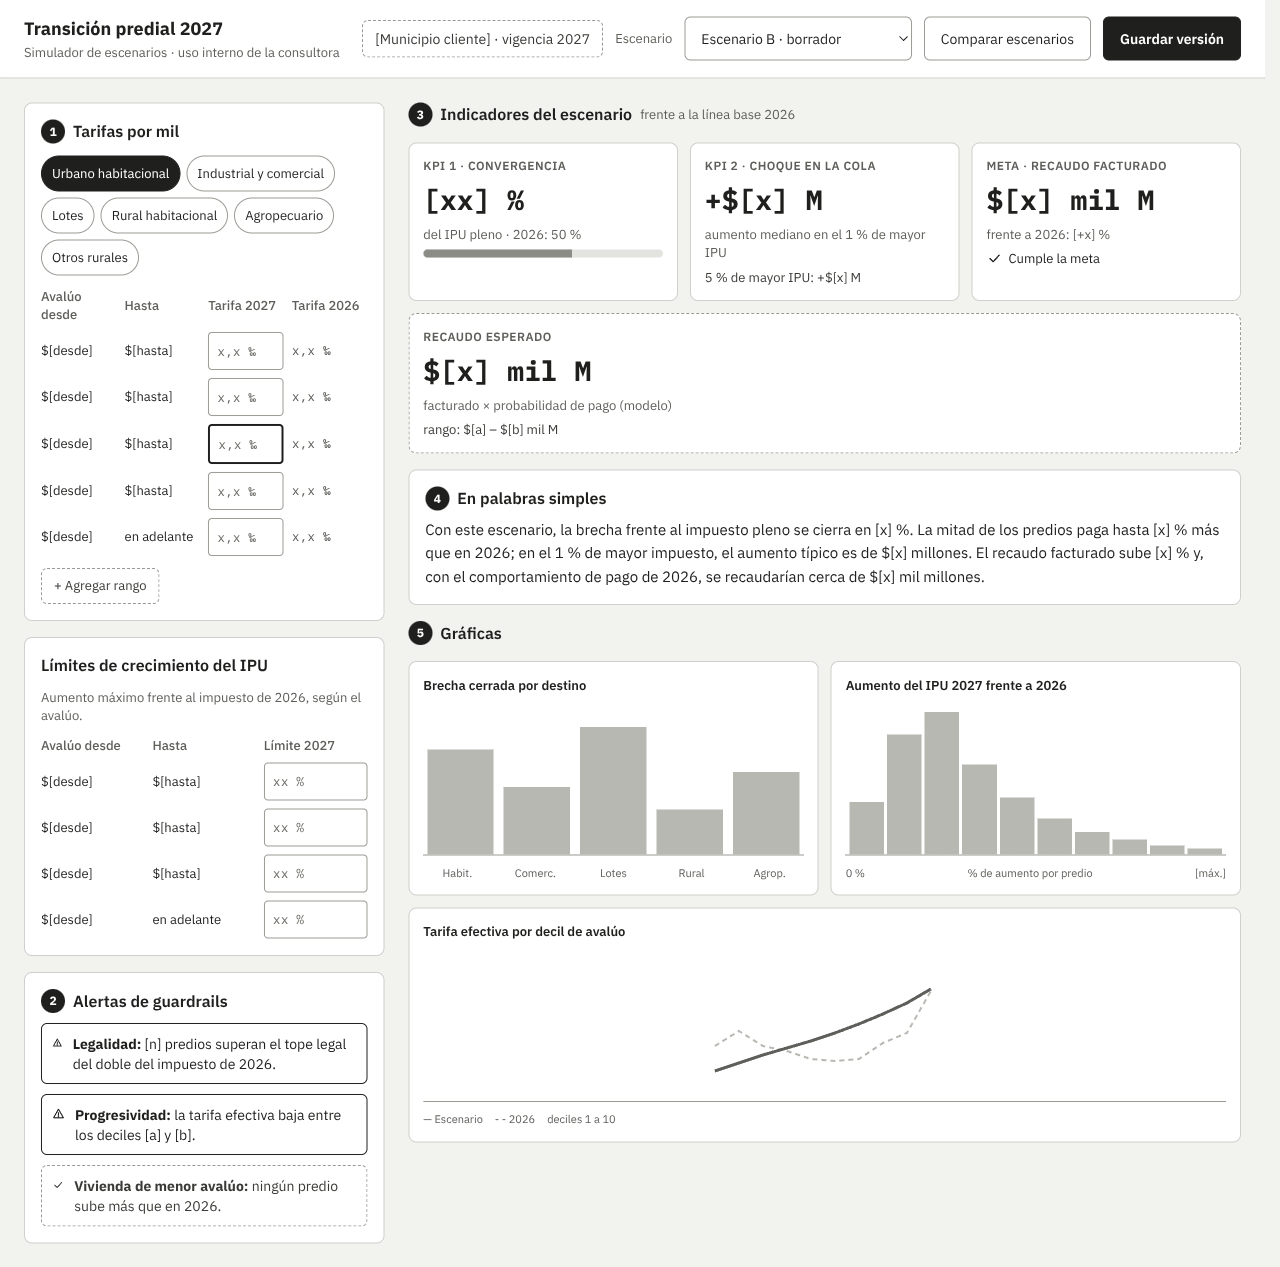
\includegraphics[width=\linewidth]{imagenes/mockup.png}
  \captionsetup{font=footnotesize,skip=3pt}
  \caption{Wireframe de la aplicación: (1) tarifas y límites; (2) alertas; (3) indicadores;
  (4) lectura en lenguaje llano; (5) gráficas. Cifras entre corchetes: marcadores.}
  \label{fig:mockup}
  \vspace{-1\baselineskip}
\end{wrapfigure}
\textbf{Dos superficies.} La decisión no se automatiza: el producto organiza la
información para que la tomen personas. Tiene una superficie interactiva, para la
consultora y las reuniones con la administración hasta el despacho del alcalde
(figura~\ref{fig:mockup}), y una exportación congelada y versionada del escenario
elegido (tablas, gráficas y textos en lenguaje llano), que sirve de insumo para el
material que se lleva al Concejo. El Concejo no opera el simulador: cambiar valores en
vivo durante el debate invitaría a tergiversar los resultados.

\textbf{Requerimientos.} Funcionales: cargar los datos de un municipio (catastro en
LADM-COL y facturación del predial) desde un formato documentado; definir tarifas por
destino y rango de avalúo y límites de crecimiento por rango; calcular en segundos el
IPU 2027 de cada predio y los indicadores de la tabla~\ref{tab:kpis}; comparar y
versionar escenarios; estimar el recaudo esperado; alertar cuando un escenario incumpla
un guardrail, y exportar el escenario congelado. No funcionales: explicabilidad en
lenguaje llano, trazabilidad de cada exportación a su escenario y sus datos, ningún dato
personal y uso exclusivo de la consultora.

\textbf{Componentes.} (1)~Un motor de escenarios determinista, que aplica las tarifas y
los topes como reglas de negocio; (2)~un modelo de \textit{machine learning} que estima
la probabilidad de que cada predio pague la vigencia, entrenado con el indicador de pago
de la facturación, y que ajusta el recaudo facturado a uno esperado; (3)~una API REST
que expone el motor, el modelo y la exportación, y (4)~una aplicación web, la superficie
interactiva. Se construirán en Python, con pandas, scikit-learn, FastAPI y Dash.

\end{espacio}

\begin{espacio}{0.35}
\section{Aspectos éticos y legales} % 10 %
% Retroalimentación (10/10): nivel máximo.
% Implicaciones éticas, de privacidad, confidencialidad, transparencia y
% regulatorias en este contexto. Las fuentes consultadas se citan con \cite{clave}
% y van en referencias.bib.
\heredado

\textbf{Protección de datos personales.} Los registros catastrales vinculan predios con personas, por lo que su tratamiento se rige por
la Ley 1581 de 2012: la alcaldía es la responsable del tratamiento y Multiaservi actúa como
encargada \cite{ley1581_2012}. El proyecto aplica la minimización desde la construcción de los
datos: el archivo de análisis no contiene nombres, documentos ni contactos de los propietarios
(los titulares quedan reducidos a conteos), los números de identificación se borran de los
textos libres, de las geometrías solo quedan medidas y de la facturación solo se leen el
impuesto y el indicador de pago. Como el número predial sigue identificando cada predio, el
archivo no es anónimo: no se publica en el repositorio, ninguna salida muestra datos de un
predio individual y el municipio no se nombra en los entregables.

\textbf{Transparencia.} Los registros catastrales y tributarios de cada predio no se publican: la Ley 1712 de 2014
exceptúa del acceso público la información que afecta la intimidad de las personas
\cite{ley1712_2014}. Lo que sí es público es la decisión: el proyecto de acuerdo y su
sustentación técnica se debaten en el Concejo y se publican con el acuerdo. Por eso, lo que
el producto exporte para esa sustentación debe ser agregado, explicable en palabras simples y
presentar el recaudo esperado como una estimación sujeta a incertidumbre, no como una
garantía.

% POR CONFIRMAR (equipo, revisión interna): compactar esta parte en una oración, quitar
% "datos de fuentes autorizadas…" y advertir que la Ley 1995 de 2019 se aplicaba por cinco
% años desde agosto de 2019 (art. 3), salvo que se confirme una prórroga.
\textbf{Legalidad tributaria y normativa catastral.} El aplicativo deberá incorporar las disposiciones legales aplicables al Impuesto Predial Unificado, 
considerando la Ley 44 de 1990 y la Ley 1995 de 2019 \cite{ley44,ley1995_2019}. Estas normas deberán analizarse conjuntamente con 
las reglas tributarias municipales vigentes y las condiciones específicas aplicables a cada predio.

Por otra parte, los datos de entrada deberán proceder de fuentes autorizadas y contar con la documentación
necesaria para interpretar sus variables y estructuras.

\textbf{Equidad tributaria y prevención de sesgos.} Un menor historial de pago en un grupo de
predios no demuestra una menor capacidad económica de sus propietarios. Por eso, el modelo de
pago solo estima el recaudo agregado, no atribuye responsabilidades individuales, y sus errores
se compararán entre grupos de predios.

\textbf{Costo político y progresividad.} Los límites al crecimiento del IPU concentran su alivio en pocos predios: el 1\,\% de los
predios con mayor brecha acumula el 47\,\% de la brecha frente al IPU pleno. Mitigar el costo
político puede, por eso, volver menos progresivo el impuesto. El producto hace visible esa
tensión con el guardrail de progresividad de la tabla~\ref{tab:kpis}, para que la decisión se
tome de forma explícita.

\end{espacio}

\begin{espacio}{0.50}
\section{Enfoque analítico} % 15 %
% Retroalimentación (15/15): nivel máximo.
% Las hipótesis o preguntas de negocio que guían la experimentación. Las técnicas
% estadísticas, de visualización y de machine learning que las responderán. Las
% métricas con las que se evaluará la calidad del modelo.
\heredado
\textbf{Preguntas de negocio.} (1)~¿Qué combinación de tarifas y límites de crecimiento para
2027 acerca más el IPU facturado al pleno (KPI~1) sin que el aumento en la cola supere lo que la
administración considere aceptable (KPI~2), cumpliendo la meta y los guardrails de la
tabla~\ref{tab:kpis}? (2)~¿Qué tan bien se puede anticipar si un predio pagará su impuesto, para
pasar del recaudo facturado al esperado? Para la segunda planteamos una hipótesis: el historial
de pago explica la mayor parte del comportamiento (pagó en 2026 el 80\,\% de quienes pagaron en
2025 y el 0,3\,\% de quienes no), y las características del predio mejoran la predicción donde
hay incertidumbre: los predios nuevos y los que dejan de pagar.

\textbf{Técnicas.} La primera pregunta se responde con el motor de escenarios, que aplica a cada
predio las tarifas y los límites de un escenario y calcula los indicadores; recorrer una malla de
escenarios muestra la frontera entre convergencia y choque sobre la que decide la administración.
La segunda se responde con
un modelo de clasificación binaria. La variable objetivo es si el predio pagó la vigencia 2026 a
la fecha de corte, y las variables son las que se conocen antes de la vigencia: el pago de 2025,
con una categoría para los predios nuevos, y el avalúo, la destinación, la condición del predio,
la zona y las áreas del catastro. Se compararán tres algoritmos, cada uno con varios conjuntos de
hiperparámetros: regresión logística y un árbol de decisión poco profundo, fáciles de explicar, y
\textit{gradient boosting}. El recaudo esperado de un escenario es
$R_{\text{esperado}}=\sum_{i} \mathit{IPU}_i\,p_i$, donde $\mathit{IPU}_i$ es el impuesto del
predio $i$ en el escenario y $p_i$ su probabilidad estimada de pago. El modelo describe asociaciones de 2026: no predice cómo reaccionarían los
contribuyentes a un aumento distinto.

\textbf{Métricas.} El motor se valida reproduciendo el IPU facturado en 2026 con las reglas del
acuerdo vigente, salvo en el 6\,\% de predios cuyo avalúo difiere entre el catastro y Hacienda.
El modelo se entrena con una partición estratificada en entrenamiento, validación y prueba, y se
evalúa en prueba con ROC-AUC para la discriminación, y con \textit{log-loss} y una curva de
calibración para la calidad de las probabilidades, que son las que entran al recaudo esperado.
Todas las métricas se comparan con una línea base, repetir el pago de 2025, y se reportan por
grupo: los predios que pagaron en 2025, los que no y los nuevos.

\end{espacio}

\begin{espacio}{0.30}
\section{Recolección de datos} % 10 %
% Retroalimentación (8,33/10, nivel 4 de 5): vacíos menores en la cobertura del
% diccionario o en la importancia de alguna fuente; el nivel 5 pide dejar claro el
% origen, el acceso y la pertinencia de cada fuente.
% Las fuentes de datos, según su estructura e importancia. El diccionario de datos
% completo va en el repositorio; aquí, solo las entidades o atributos más relevantes.
\heredado
Los datos vienen de dos fuentes del municipio y se integran en un solo archivo con un predio por
fila. La primera es el levantamiento catastral, producido por el operador catastral y entregado
por el gestor catastral como un archivo de transferencia
\enlace{https://www.interlis.ch/en}{INTERLIS} en el modelo
\enlace{https://www.igac.gov.co/catastro-multiproposito/ladmcol}{LADM-COL}. Se cargó
en PostgreSQL con \enlace{https://github.com/claeis/ili2db}{ili2pg} (217 tablas) y se podó a las 45 tablas con contenido útil; una consulta
SQL arma cada predio con sus terrenos, construcciones, unidades y titulares (estos, reducidos a
conteos), y un programa en Python lo escribe en un archivo parquet con un esquema fijo. La
segunda es el comparativo de facturación del impuesto predial de 2025 y 2026, exportado por la
Secretaría de Hacienda: de él solo se toman el impuesto facturado en 2026 y si el predio pagó en
2025 y en 2026, unidos por el número predial. El catastro es la fuente de todo atributo
catastral, y el archivo final tiene 22\,220 predios y ningún dato personal.

Los atributos principales son el avalúo catastral, la destinación económica, la condición del
predio (no sometido a propiedad horizontal, propiedad horizontal, condominio o informal), la zona
urbana o rural, las áreas de terreno y construida, el uso, la edad y la altura de las
construcciones, el resultado de la visita de campo, las novedades del número predial frente al
catastro anterior y, de la facturación, el impuesto facturado y el pago. El proceso completo está
en el \repo{datos/predios/README.md}{repositorio}, con el
\repo{datos/predios/diccionario/diccionario-de-datos.pdf}{diccionario de datos}. El archivo no se
publica; está en el \enlace{\urldatos}{almacenamiento de la Universidad}, con acceso restringido.

\end{espacio}

\begin{espacio}{0.90}
\section{Entendimiento de los datos} % 35 %
% Retroalimentación (26,25/35, nivel 4 de 5): falta profundidad en el análisis
% multivariado, la evaluación de suficiencia o la interpretación desde el negocio.
% El nivel 5 nombra también el desbalance y los duplicados.
% Los resultados más importantes del análisis exploratorio y de la calidad de los
% datos. Debe notarse el uso de técnicas univariadas y multivariadas, gráficas y
% no gráficas. El notebook completo se enlaza con \repo.
% Reescrita para la entrega final según la retroalimentación (issue #1): análisis
% multivariado sobre el pago, desbalance, sesgo del cruce, suficiencia por grupo y
% qué implica cada hallazgo. Pendiente de revisión del equipo.
El \repo{entrega-2/notebooks/06-entendimiento-de-los-datos.ipynb}{notebook de entendimiento de
los datos} analiza los 22\,220 predios del levantamiento y los 19\,150 que Hacienda facturó en
2026. Usa estadísticos de forma, Box-Cox, frecuencias, tablas cruzadas con chi-cuadrado y V de
Cramér, Mann-Whitney por régimen, PCA, regresión descriptiva y AUC univariada, con histogramas,
cajas, mapas de calor y un biplot.

\textbf{Avalúo.} Es muy asimétrico (mediana de 236 millones, asimetría de 37,7) y se analiza en
escala logarítmica (Box-Cox $\lambda \approx 0$). Depende casi solo del tamaño: el primer
componente del PCA se correlaciona 0,92 con él. Para el motor, el avalúo es coherente entre
predios comparables.

\textbf{Pago.} Pagó la vigencia 2026 el 64\,\% de los predios facturados. El historial de 2025
domina (V de Cramér = 0,57), y las características del catastro pesan donde el historial no
decide: entre los predios sin registro de 2025, el decil de avalúo se asocia con el pago
(V = 0,31) más del doble que entre los que pagaron (0,13), y pagó el 50\,\% de los predios nuevos
frente al 61\,\% de los desenglobes. Para el modelo: el historial y la novedad del número predial
entran como variables, con interacciones entre ellas y el resto.

\begin{destacado}
\textbf{Pagó en 2026 el 80,3\,\% de quienes pagaron 2025 y el 0,3\,\% de quienes no.} La
incertidumbre está en el 20\,\% que dejó de pagar y en los 3\,927 predios sin registro de 2025.
\end{destacado}

\textbf{Desbalance.} En total es leve (64\,\% y 36\,\%), pero entre quienes no pagaron 2025 solo
9 de 2\,703 pagaron. La partición se estratifica por pago y por historial, y las métricas se
reportan por grupo. \textbf{Concentración.} El 1\,\% de los predios con mayor impuesto factura el
46,8\,\% del total: el KPI~2 y el recaudo esperado dependen de pocos predios.

\begin{table}[H]
  \centering
  \caption{Principales problemas de calidad y su tratamiento en la preparación.}
  \label{tab:calidad}
  \small
  \begin{tabular}{@{}>{\raggedright\arraybackslash}p{0.44\linewidth}
                     >{\raggedleft\arraybackslash}p{0.10\linewidth}
                     >{\raggedright\arraybackslash}p{0.40\linewidth}@{}}
    \toprule
    Problema & Predios & Tratamiento \\
    \midrule
    Fecha de visita de relleno, todas incompletas & 9\,010 & Faltante; se usa la visita efectiva \\
    Año de construcción 2000 de relleno & 3\,322 & Faltante, con un indicador \\
    Avalúo igual a 0 & 2\,335 & Faltante, con un indicador \\
    Unidades de PH sin terreno ni pisos propios & 10\,993 & Terreno y pisos de su matriz \\
    Predios del catastro sin facturación & 2\,888 & Fuera del modelo \\
    \bottomrule
  \end{tabular}
\end{table}

\textbf{Calidad y suficiencia.} La bitácora del notebook registra 32 problemas (tabla~\ref{tab:calidad});
los formatos y dominios no tienen errores. El cruce con la facturación no sesga la muestra: 746
de los 748 predios individuales sin facturar son predios cancelados en la actualización. Cada
grupo del historial tiene miles de predios, y todas las variables candidatas tienen menos de
5\,\% de faltantes, salvo el año de construcción (30\,\%). Los límites son el pago cortado a la
fecha de extracción y los 270 predios que Hacienda liquidó con un avalúo distinto del catastral.

\end{espacio}

\begin{espacio}{0.30}
\section{Conclusiones iniciales} % 10 %
% Retroalimentación (5/10, nivel 3 de 5): "pocos insights reales" y acciones
% próximas "genéricas o poco conectadas con los hallazgos". Es la que más hay que
% rehacer: insights para el negocio y acciones concretas que salgan de ellos.
% Primeras conclusiones e insights, y las acciones que siguen.
\heredado
Los datos alcanzan para las dos preguntas: la facturación cubre el 87\,\% del levantamiento y el
historial de pago anticipa casi todo el comportamiento. El 10\,\% de los predios con mayor
impuesto factura el 81\,\% del total, y en él recae el KPI~2. Sigue validar el motor con las
tarifas vigentes.

\end{espacio}

\begin{espacio}{1.55}
\section{Preparación de datos} % 20 %
% El proceso de preparación y evidencia de los datos preparados. Las
% transformaciones: nuevas características, codificación de categóricas,
% normalización, estandarización, imputación de faltantes, etc. Recomendado: un
% diagrama de bloques funcional de los procesos (entrega-2/diagramas/preparacion.mmd).
% Detalle en el notebook 08.
Pendiente: el proceso de preparación, las transformaciones y la evidencia de los datos
preparados, con enlace al
\repo{entrega-2/notebooks/08-preparacion-de-datos.ipynb}{notebook de preparación de los datos}.

\end{espacio}

\begin{espacio}{0.50}
\section{Estrategia de validación y selección del modelo} % 5 %
% La estrategia de experimentación para entrenar y seleccionar el mejor modelo. La
% partición en entrenamiento, validación y prueba, y un reporte breve de que los
% subconjuntos conservan la distribución del conjunto original. Detalle en el notebook 09.
Pendiente: la estrategia de experimentación, la partición y la verificación de las
distribuciones, con enlace al
\repo{entrega-2/notebooks/09-estrategia-de-validacion.ipynb}{notebook de validación}.

\end{espacio}

\begin{espacio}{1.60}
\section{Construcción y evaluación del modelo} % 20 %
% Modelos con al menos tres algoritmos y distintos conjuntos de hiperparámetros.
% Evaluación cuantitativa con las métricas del enfoque analítico (sección 4) y
% cualitativa en la medida de lo posible. Oportunidades de mejora. Detalle en el
% notebook 10.
Pendiente: los algoritmos y sus hiperparámetros, la evaluación frente a la línea base y
las oportunidades de mejora, con enlace al
\repo{entrega-2/notebooks/10-construccion-y-evaluacion-del-modelo.ipynb}{notebook de
modelado}.

\end{espacio}

\begin{espacio}{1.55}
\section{Producto de datos} % 20 %
% El prototipo funcional con el mejor modelo, la API REST, la aplicación web y/o el
% dashboard. El mecanismo de despliegue. El diagrama de arquitectura
% (entrega-2/diagramas/arquitectura.mmd).
Pendiente: el prototipo, su despliegue y su arquitectura, con enlace a
\repo{entrega-2/producto/README.md}{la carpeta del producto}.

\end{espacio}

\begin{espacio}{1.05}
\section{Retroalimentación de la organización} % 15 %
% La bitácora de al menos tres interacciones con los stakeholders durante el
% semestre, con los acuerdos sobre la problemática, el producto de datos, el
% enfoque analítico y los resultados. La presentación de los resultados y del
% producto, con la retroalimentación recibida y los próximos pasos.
Pendiente: el resumen de las interacciones y de la presentación final, con enlace a la
\repo{entrega-2/bitacora-stakeholders.md}{bitácora}.

\end{espacio}

\begin{espacio}{1.25}
\section{Conclusiones} % 15 %
% Resumen ejecutivo de los resultados más relevantes. ¿Se cumplieron los objetivos?
% ¿Cuáles fueron las mayores dificultades? ¿Cómo se impactarían los KPIs con el
% producto en uso real? ¿Qué condiciones deberían tener los datos para obtener
% mejores resultados? ¿El mejor modelo es suficiente para resolver el problema?
Pendiente: el resumen ejecutivo y la respuesta a las cinco preguntas del enunciado.

\end{espacio}

\begin{espacio}[referencias]{0.65}
\printbibliography
\end{espacio}

\end{document}
